% Options for packages loaded elsewhere
\PassOptionsToPackage{unicode}{hyperref}
\PassOptionsToPackage{hyphens}{url}
%
\documentclass[
]{article}
\usepackage{amsmath,amssymb}
\usepackage{iftex}
\ifPDFTeX
  \usepackage[T1]{fontenc}
  \usepackage[utf8]{inputenc}
  \usepackage{textcomp} % provide euro and other symbols
\else % if luatex or xetex
  \usepackage{unicode-math} % this also loads fontspec
  \defaultfontfeatures{Scale=MatchLowercase}
  \defaultfontfeatures[\rmfamily]{Ligatures=TeX,Scale=1}
\fi
\usepackage{lmodern}
\ifPDFTeX\else
  % xetex/luatex font selection
\fi
% Use upquote if available, for straight quotes in verbatim environments
\IfFileExists{upquote.sty}{\usepackage{upquote}}{}
\IfFileExists{microtype.sty}{% use microtype if available
  \usepackage[]{microtype}
  \UseMicrotypeSet[protrusion]{basicmath} % disable protrusion for tt fonts
}{}
\makeatletter
\@ifundefined{KOMAClassName}{% if non-KOMA class
  \IfFileExists{parskip.sty}{%
    \usepackage{parskip}
  }{% else
    \setlength{\parindent}{0pt}
    \setlength{\parskip}{6pt plus 2pt minus 1pt}}
}{% if KOMA class
  \KOMAoptions{parskip=half}}
\makeatother
\usepackage{xcolor}
\usepackage[margin=1in]{geometry}
\usepackage{color}
\usepackage{fancyvrb}
\newcommand{\VerbBar}{|}
\newcommand{\VERB}{\Verb[commandchars=\\\{\}]}
\DefineVerbatimEnvironment{Highlighting}{Verbatim}{commandchars=\\\{\}}
% Add ',fontsize=\small' for more characters per line
\usepackage{framed}
\definecolor{shadecolor}{RGB}{248,248,248}
\newenvironment{Shaded}{\begin{snugshade}}{\end{snugshade}}
\newcommand{\AlertTok}[1]{\textcolor[rgb]{0.94,0.16,0.16}{#1}}
\newcommand{\AnnotationTok}[1]{\textcolor[rgb]{0.56,0.35,0.01}{\textbf{\textit{#1}}}}
\newcommand{\AttributeTok}[1]{\textcolor[rgb]{0.13,0.29,0.53}{#1}}
\newcommand{\BaseNTok}[1]{\textcolor[rgb]{0.00,0.00,0.81}{#1}}
\newcommand{\BuiltInTok}[1]{#1}
\newcommand{\CharTok}[1]{\textcolor[rgb]{0.31,0.60,0.02}{#1}}
\newcommand{\CommentTok}[1]{\textcolor[rgb]{0.56,0.35,0.01}{\textit{#1}}}
\newcommand{\CommentVarTok}[1]{\textcolor[rgb]{0.56,0.35,0.01}{\textbf{\textit{#1}}}}
\newcommand{\ConstantTok}[1]{\textcolor[rgb]{0.56,0.35,0.01}{#1}}
\newcommand{\ControlFlowTok}[1]{\textcolor[rgb]{0.13,0.29,0.53}{\textbf{#1}}}
\newcommand{\DataTypeTok}[1]{\textcolor[rgb]{0.13,0.29,0.53}{#1}}
\newcommand{\DecValTok}[1]{\textcolor[rgb]{0.00,0.00,0.81}{#1}}
\newcommand{\DocumentationTok}[1]{\textcolor[rgb]{0.56,0.35,0.01}{\textbf{\textit{#1}}}}
\newcommand{\ErrorTok}[1]{\textcolor[rgb]{0.64,0.00,0.00}{\textbf{#1}}}
\newcommand{\ExtensionTok}[1]{#1}
\newcommand{\FloatTok}[1]{\textcolor[rgb]{0.00,0.00,0.81}{#1}}
\newcommand{\FunctionTok}[1]{\textcolor[rgb]{0.13,0.29,0.53}{\textbf{#1}}}
\newcommand{\ImportTok}[1]{#1}
\newcommand{\InformationTok}[1]{\textcolor[rgb]{0.56,0.35,0.01}{\textbf{\textit{#1}}}}
\newcommand{\KeywordTok}[1]{\textcolor[rgb]{0.13,0.29,0.53}{\textbf{#1}}}
\newcommand{\NormalTok}[1]{#1}
\newcommand{\OperatorTok}[1]{\textcolor[rgb]{0.81,0.36,0.00}{\textbf{#1}}}
\newcommand{\OtherTok}[1]{\textcolor[rgb]{0.56,0.35,0.01}{#1}}
\newcommand{\PreprocessorTok}[1]{\textcolor[rgb]{0.56,0.35,0.01}{\textit{#1}}}
\newcommand{\RegionMarkerTok}[1]{#1}
\newcommand{\SpecialCharTok}[1]{\textcolor[rgb]{0.81,0.36,0.00}{\textbf{#1}}}
\newcommand{\SpecialStringTok}[1]{\textcolor[rgb]{0.31,0.60,0.02}{#1}}
\newcommand{\StringTok}[1]{\textcolor[rgb]{0.31,0.60,0.02}{#1}}
\newcommand{\VariableTok}[1]{\textcolor[rgb]{0.00,0.00,0.00}{#1}}
\newcommand{\VerbatimStringTok}[1]{\textcolor[rgb]{0.31,0.60,0.02}{#1}}
\newcommand{\WarningTok}[1]{\textcolor[rgb]{0.56,0.35,0.01}{\textbf{\textit{#1}}}}
\usepackage{graphicx}
\makeatletter
\def\maxwidth{\ifdim\Gin@nat@width>\linewidth\linewidth\else\Gin@nat@width\fi}
\def\maxheight{\ifdim\Gin@nat@height>\textheight\textheight\else\Gin@nat@height\fi}
\makeatother
% Scale images if necessary, so that they will not overflow the page
% margins by default, and it is still possible to overwrite the defaults
% using explicit options in \includegraphics[width, height, ...]{}
\setkeys{Gin}{width=\maxwidth,height=\maxheight,keepaspectratio}
% Set default figure placement to htbp
\makeatletter
\def\fps@figure{htbp}
\makeatother
\setlength{\emergencystretch}{3em} % prevent overfull lines
\providecommand{\tightlist}{%
  \setlength{\itemsep}{0pt}\setlength{\parskip}{0pt}}
\setcounter{secnumdepth}{-\maxdimen} % remove section numbering
\ifLuaTeX
  \usepackage{selnolig}  % disable illegal ligatures
\fi
\IfFileExists{bookmark.sty}{\usepackage{bookmark}}{\usepackage{hyperref}}
\IfFileExists{xurl.sty}{\usepackage{xurl}}{} % add URL line breaks if available
\urlstyle{same}
\hypersetup{
  pdftitle={HUDM6052 Psychometric II Homework\_02},
  pdfauthor={Chenguang Pan (cp3280@tc.columbia.edu)},
  hidelinks,
  pdfcreator={LaTeX via pandoc}}

\title{HUDM6052 Psychometric II Homework\_02}
\author{Chenguang Pan
(\href{mailto:cp3280@tc.columbia.edu}{\nolinkurl{cp3280@tc.columbia.edu}})}
\date{2023-10-27}

\begin{document}
\maketitle

\setcounter{tocdepth}{4}
\tableofcontents

\hypertarget{q1}{%
\subsection{Q1}\label{q1}}

\emph{Find the maximum discrimination for 1PL, 2PL, and 3PL logistic
models\ldots{}}

\textbf{My Solution:}\\
\textbf{2PL MODEL}

I begin with a 2PL model since 1PL is a special case of 2PL. The
ultimate purpose is to get the slope function \(S(\theta)\) and take the
first derivative of this slope function and let it equal to 0 to get the
local maximum. One should notice that the slope function \(S(\theta)\)
is actually the first derivative of the 2PL function \(P(\theta)\).
Follow this idea, I derive the conclusion step by step:

For the 2PL model, \[P(\theta)=\frac{1}{1+e^{-\alpha(\theta-\beta)}},\]
let \(Z = \alpha(\theta-\beta)\), \(U = e^{-Z}\), and then
\(P = \frac{1}{1+U}\). Using the chain rule and take the partial
derivative on \(\theta\), one can have
\[\frac{\partial P}{\partial \theta}=\frac{\partial P}{\partial U}\frac{\partial U}{\partial Z}\frac{\partial Z}{\partial \theta}. \]
Since \[\frac{\partial P}{\partial U}=\frac{-1}{(1+U^2)},\]
\[\frac{\partial U}{\partial Z}=-e^{-Z},\] and
\[\frac{\partial Z}{\partial \theta}= \alpha,\] plug all three partial
derivatives into the overall equation. One can have the slope function
\[S(\theta)=\frac{\partial P}{\partial \theta}=\frac{\alpha e^{-z}}{(1 + e^{-z})^2}.\]
Next, continue to take the first derivative of this slope function, one
can have
\[S'(\theta)=\frac{\partial^2 P}{\partial \theta^2}=\alpha^2[\frac{-2U}{(1+U)^3}+\frac{1}{(1+U)^2}](-U),\]
\[S'(\theta)=\frac{\partial^2 P}{\partial \theta^2}=\alpha^2[\frac{U(1-U)}{(1+U)^3}].\]

Let it equal to 0, and one can have \[U=e^{-\alpha(\theta-\beta)}=1.\]
It is not difficult to have the final solution \[\theta = \beta.\] The
maximum value of discrimination of a 2PL model is at the point
\(\theta =\beta\).\\
Therefore, the maximum of the 2PL model's slope is
\[\frac{1}{4}\alpha\].

\textbf{1PL MODEL}

Since the 1PL is a special case of 2PL, plug the \(\alpha = 1\) into the
partial derivative of slope function \(S'(\theta)\) above. One can
easily have same conclusion that the maximum of slope of 1PL model is at
the point \(\theta = \beta\).\\
Therefore, the maximum of the 1PL model's slope is \(\frac{1}{4}.\)

\textbf{3PL MODEL}\\
For the 3PL model, follow the idea above. It is not difficult to get the
slope function \[S(\theta)=\frac{\alpha (1-c) e^{-z}}{(1 + e^{-z})^2}.\]
Plug the \(\theta=\beta\), one can easily have the maximum slope is
\[\frac{1}{4}\alpha(1-c).\]

\hypertarget{q2}{%
\subsection{Q2}\label{q2}}

\emph{Let the discrimination, difficulty and guessing parameters of five
items be\ldots{}}

\textbf{My Solution:}\\
First, I write a 3PL model function:

\begin{Shaded}
\begin{Highlighting}[]
\SpecialCharTok{\textgreater{}} \CommentTok{\# items\textquotesingle{} discrimination}
\ErrorTok{\textgreater{}}\NormalTok{ a\_ }\OtherTok{\textless{}{-}} \FunctionTok{c}\NormalTok{(}\FloatTok{0.5}\NormalTok{,}\DecValTok{1}\NormalTok{,}\FloatTok{1.5}\NormalTok{,}\FloatTok{2.5}\NormalTok{,}\DecValTok{1}\NormalTok{)}
\SpecialCharTok{\textgreater{}} \CommentTok{\# items\textquotesingle{} difficulty levels}
\ErrorTok{\textgreater{}}\NormalTok{ b\_ }\OtherTok{\textless{}{-}} \FunctionTok{c}\NormalTok{(}\SpecialCharTok{{-}}\DecValTok{1}\NormalTok{,}\SpecialCharTok{{-}}\FloatTok{0.5}\NormalTok{,}\DecValTok{0}\NormalTok{,}\FloatTok{0.5}\NormalTok{,}\DecValTok{1}\NormalTok{)}
\SpecialCharTok{\textgreater{}} \CommentTok{\# items\textquotesingle{}s guessing parameters}
\ErrorTok{\textgreater{}}\NormalTok{ c\_ }\OtherTok{\textless{}{-}} \FunctionTok{c}\NormalTok{(}\DecValTok{0}\NormalTok{,}\FloatTok{0.1}\NormalTok{,}\FloatTok{0.15}\NormalTok{,}\FloatTok{0.05}\NormalTok{,}\FloatTok{0.32}\NormalTok{)}
\SpecialCharTok{\textgreater{}} \CommentTok{\# trait vector}
\ErrorTok{\textgreater{}}\NormalTok{ theta\_ }\OtherTok{\textless{}{-}} \FunctionTok{c}\NormalTok{(}\SpecialCharTok{{-}}\FloatTok{2.0}\NormalTok{, }\SpecialCharTok{{-}}\FloatTok{1.0}\NormalTok{, }\DecValTok{0}\NormalTok{,}\DecValTok{1}\NormalTok{,}\DecValTok{2}\NormalTok{)}
\SpecialCharTok{\textgreater{}} \CommentTok{\# write a 3PL model}
\ErrorTok{\textgreater{}}\NormalTok{ irt\_3pl }\OtherTok{\textless{}{-}} \ControlFlowTok{function}\NormalTok{(theta,a,b,c)\{}
\SpecialCharTok{+}\NormalTok{   z }\OtherTok{\textless{}{-}} \FloatTok{1.702}\SpecialCharTok{*}\NormalTok{a}\SpecialCharTok{*}\NormalTok{(theta }\SpecialCharTok{{-}}\NormalTok{ b)}
\SpecialCharTok{+}\NormalTok{   output }\OtherTok{\textless{}{-}}\NormalTok{ c }\SpecialCharTok{+}\NormalTok{ (}\DecValTok{1}\SpecialCharTok{{-}}\NormalTok{c)}\SpecialCharTok{/}\NormalTok{(}\DecValTok{1}\SpecialCharTok{+}\FunctionTok{exp}\NormalTok{(}\SpecialCharTok{{-}}\NormalTok{z))}
\SpecialCharTok{+}   \FunctionTok{return}\NormalTok{(output)}
\SpecialCharTok{+}\NormalTok{ \}}
\end{Highlighting}
\end{Shaded}

Next, for each test-taker (i.e., each trait), get the required values
iteratively.

\begin{Shaded}
\begin{Highlighting}[]
\SpecialCharTok{\textgreater{}} \CommentTok{\# using a for{-}loop to get the values}
\ErrorTok{\textgreater{}} \ControlFlowTok{for}\NormalTok{ (j }\ControlFlowTok{in} \DecValTok{1}\SpecialCharTok{:}\DecValTok{5}\NormalTok{) \{}
\SpecialCharTok{+}   \CommentTok{\#print(paste0("{-}{-}{-}{-}{-}{-}{-}{-}{-}{-}{-}{-}{-}For the theta =", theta\_[j]," : {-}{-}{-}{-}{-}{-}{-}{-}{-}{-}{-}{-}{-}"))}
\SpecialCharTok{+}\NormalTok{   exp\_cor }\OtherTok{\textless{}{-}} \DecValTok{0}
\SpecialCharTok{+}   \ControlFlowTok{for}\NormalTok{ (i }\ControlFlowTok{in} \DecValTok{1}\SpecialCharTok{:}\DecValTok{5}\NormalTok{) \{}
\SpecialCharTok{+}     \CommentTok{\#print(paste0("{-}{-}{-}{-}{-}For the item i=", i," : {-}{-}{-}{-}{-}"))}
\SpecialCharTok{+}\NormalTok{     P }\OtherTok{\textless{}{-}} \FunctionTok{irt\_3pl}\NormalTok{(}\AttributeTok{theta=}\NormalTok{ theta\_[j], }
\SpecialCharTok{+}                  \AttributeTok{a=}\NormalTok{a\_[i], }\AttributeTok{b=}\NormalTok{b\_[i], }\AttributeTok{c=}\NormalTok{c\_[i])}
\SpecialCharTok{+}\NormalTok{     Q }\OtherTok{\textless{}{-}} \DecValTok{1}\SpecialCharTok{{-}}\NormalTok{P}
\SpecialCharTok{+}     \CommentTok{\# get the odds}
\SpecialCharTok{+}\NormalTok{     odds }\OtherTok{\textless{}{-}} \FunctionTok{round}\NormalTok{(P}\SpecialCharTok{/}\NormalTok{Q,}\DecValTok{3}\NormalTok{)}
\SpecialCharTok{+}     \CommentTok{\# get the logit}
\SpecialCharTok{+}\NormalTok{     logit }\OtherTok{\textless{}{-}} \FunctionTok{round}\NormalTok{(}\FunctionTok{log}\NormalTok{(odds),}\DecValTok{3}\NormalTok{)    }
\SpecialCharTok{+}     \CommentTok{\# get the expected total score}
\SpecialCharTok{+}\NormalTok{     exp\_cor }\OtherTok{\textless{}{-}}\NormalTok{ exp\_cor }\SpecialCharTok{+}\NormalTok{ P}
\SpecialCharTok{+}     \CommentTok{\# print the results for this student}
\SpecialCharTok{+}     \CommentTok{\#print(paste0("Odds: ", odds," ."))}
\SpecialCharTok{+}     \CommentTok{\#print(paste0("Logit:", logit," ."))}
\SpecialCharTok{+}\NormalTok{   \}}
\SpecialCharTok{+}   \CommentTok{\# get the expected proportion of correct}
\SpecialCharTok{+}\NormalTok{   prop }\OtherTok{\textless{}{-}} \FunctionTok{round}\NormalTok{(exp\_cor}\SpecialCharTok{/}\DecValTok{5}\NormalTok{,}\DecValTok{3}\NormalTok{)}
\SpecialCharTok{+}   \CommentTok{\#print(paste0("Expected Correct \#:", exp\_cor," ."))}
\SpecialCharTok{+}   \CommentTok{\#print(paste0("Expected Correct proportion:", prop," ."))}
\SpecialCharTok{+}\NormalTok{ \}}
\end{Highlighting}
\end{Shaded}

To make the layout good-looking, I loaded the results into a table as
followed.

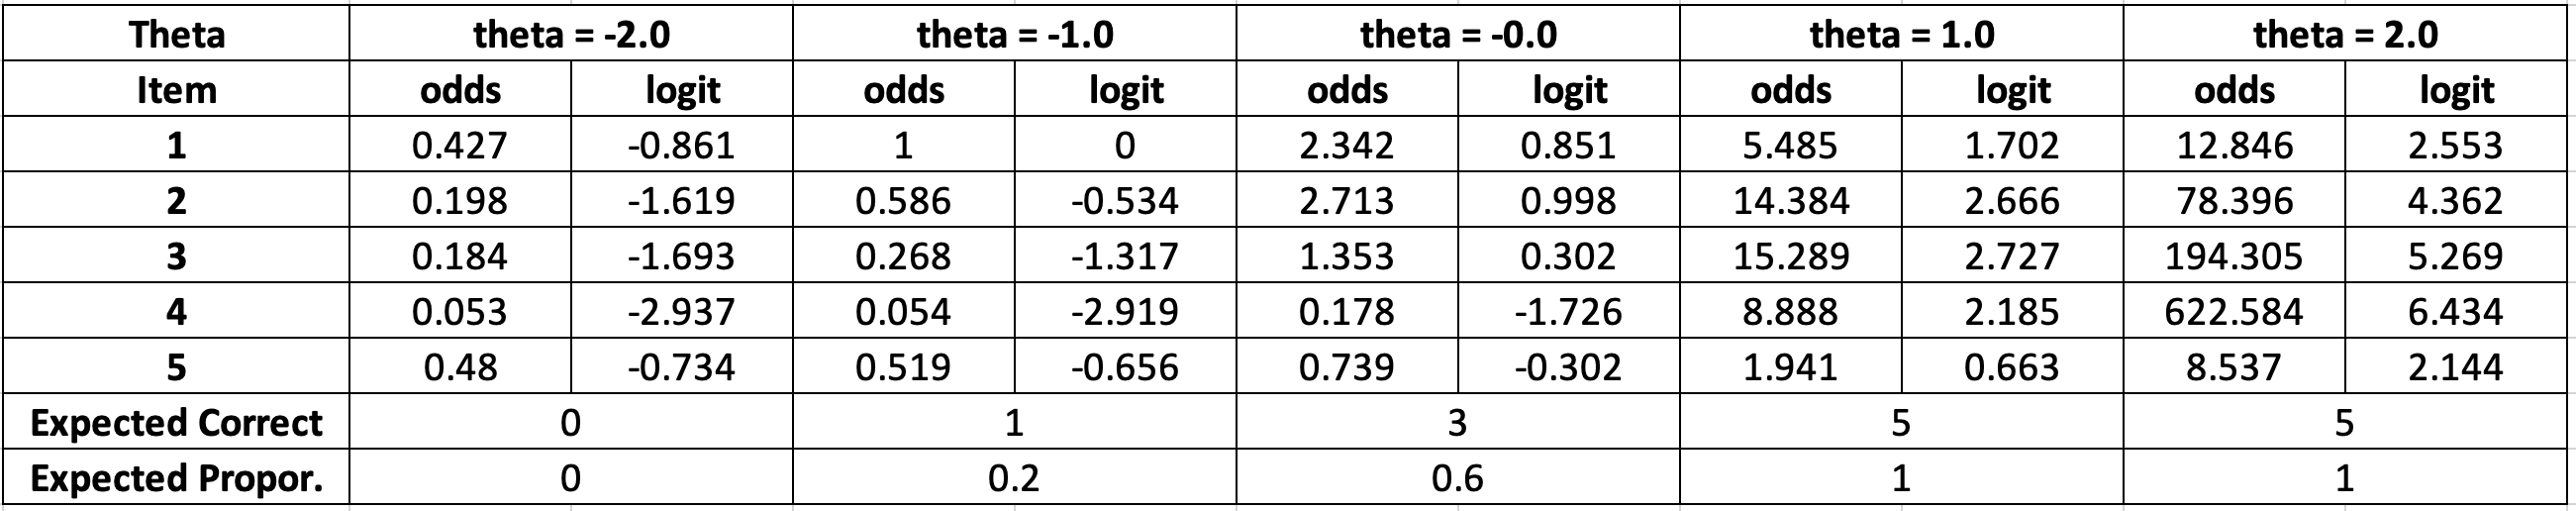
\includegraphics{table_1.png}

\hypertarget{q3-part-a}{%
\subsection{Q3-Part a}\label{q3-part-a}}

\emph{Find the maximum likelihood estimates of the item parameters
under\ldots{}}

\textbf{My Solution}

\begin{Shaded}
\begin{Highlighting}[]
\SpecialCharTok{\textgreater{}} \CommentTok{\# load the given values}
\ErrorTok{\textgreater{}} \DocumentationTok{\#\# the assumed theta\_j}
\ErrorTok{\textgreater{}}\NormalTok{ theta\_set }\OtherTok{\textless{}{-}} \FunctionTok{seq}\NormalTok{(}\SpecialCharTok{{-}}\DecValTok{3}\NormalTok{,}\DecValTok{3}\NormalTok{,}\AttributeTok{by =}\FloatTok{0.5}\NormalTok{)}
\SpecialCharTok{\textgreater{}} \DocumentationTok{\#\# number of correct responses for each theta\_j}
\ErrorTok{\textgreater{}}\NormalTok{ r\_set }\OtherTok{\textless{}{-}} \FunctionTok{c}\NormalTok{(}\DecValTok{0}\NormalTok{,}\DecValTok{0}\NormalTok{,}\DecValTok{1}\NormalTok{,}\DecValTok{2}\NormalTok{,}\DecValTok{3}\NormalTok{,}\DecValTok{4}\NormalTok{,}\DecValTok{5}\NormalTok{,}\DecValTok{6}\NormalTok{,}\DecValTok{4}\NormalTok{,}\DecValTok{4}\NormalTok{,}\DecValTok{4}\NormalTok{,}\DecValTok{2}\NormalTok{,}\DecValTok{1}\NormalTok{)}
\SpecialCharTok{\textgreater{}} \DocumentationTok{\#\# number of respondents for each theta\_j}
\ErrorTok{\textgreater{}}\NormalTok{ f\_set }\OtherTok{\textless{}{-}} \FunctionTok{c}\NormalTok{(}\DecValTok{1}\NormalTok{,}\DecValTok{2}\NormalTok{,}\DecValTok{4}\NormalTok{,}\DecValTok{7}\NormalTok{,}\DecValTok{8}\NormalTok{,}\DecValTok{9}\NormalTok{,}\DecValTok{10}\NormalTok{,}\DecValTok{8}\NormalTok{,}\DecValTok{6}\NormalTok{,}\DecValTok{5}\NormalTok{,}\DecValTok{5}\NormalTok{,}\DecValTok{2}\NormalTok{,}\DecValTok{1}\NormalTok{)}
\SpecialCharTok{\textgreater{}} 
\ErrorTok{\textgreater{}} \CommentTok{\# get the proportion of correct responses for each theta\_j}
\ErrorTok{\textgreater{}}\NormalTok{ p\_set }\OtherTok{\textless{}{-}}\NormalTok{ r\_set}\SpecialCharTok{/}\NormalTok{f\_set}
\SpecialCharTok{\textgreater{}} 
\ErrorTok{\textgreater{}} \CommentTok{\# to count the iteration times}
\ErrorTok{\textgreater{}}\NormalTok{ iter\_time }\OtherTok{\textless{}{-}} \DecValTok{0}
\SpecialCharTok{\textgreater{}}\NormalTok{ deltas }\OtherTok{\textless{}{-}} \FunctionTok{t}\NormalTok{(}\FunctionTok{t}\NormalTok{(}\FunctionTok{c}\NormalTok{(}\DecValTok{10}\NormalTok{,}\DecValTok{10}\NormalTok{)))}
\SpecialCharTok{\textgreater{}}\NormalTok{ zeta }\OtherTok{\textless{}{-}} \DecValTok{0}
\SpecialCharTok{\textgreater{}}\NormalTok{ lambda }\OtherTok{\textless{}{-}} \FloatTok{1.0}
\SpecialCharTok{\textgreater{}} 
\ErrorTok{\textgreater{}} \ControlFlowTok{while}\NormalTok{((}\FunctionTok{abs}\NormalTok{(deltas[}\DecValTok{1}\NormalTok{,}\DecValTok{1}\NormalTok{])}\SpecialCharTok{\textgreater{}}\FloatTok{0.005}\NormalTok{) }\SpecialCharTok{\&}\NormalTok{ (}\FunctionTok{abs}\NormalTok{(deltas[}\DecValTok{2}\NormalTok{,}\DecValTok{1}\NormalTok{])}\SpecialCharTok{\textgreater{}}\FloatTok{0.005}\NormalTok{)) \{}
\SpecialCharTok{+}   \CommentTok{\# set the initial value}
\SpecialCharTok{+}\NormalTok{   iter\_time }\OtherTok{\textless{}{-}}\NormalTok{ iter\_time}\SpecialCharTok{+}\DecValTok{1}
\SpecialCharTok{+}   \CommentTok{\# define the 2PL model:}
\SpecialCharTok{+}   \CommentTok{\# note, both the input and output are vectors rather than scalars}
\SpecialCharTok{+}\NormalTok{   P }\OtherTok{\textless{}{-}} \DecValTok{1}\SpecialCharTok{/}\NormalTok{(}\DecValTok{1}\SpecialCharTok{+}\FunctionTok{exp}\NormalTok{(}\SpecialCharTok{{-}}\NormalTok{(zeta}\SpecialCharTok{+}\NormalTok{lambda}\SpecialCharTok{*}\NormalTok{theta\_set)))}
\SpecialCharTok{+}\NormalTok{   Q }\OtherTok{\textless{}{-}} \DecValTok{1}\SpecialCharTok{{-}}\NormalTok{P}
\SpecialCharTok{+}   
\SpecialCharTok{+}   \CommentTok{\# define the weight in case of using normal ogive in the future}
\SpecialCharTok{+}\NormalTok{   W }\OtherTok{\textless{}{-}}\NormalTok{ P}\SpecialCharTok{*}\NormalTok{Q}
\SpecialCharTok{+}   
\SpecialCharTok{+}   \CommentTok{\# Define the L1, L11, L2, L22, L12}
\SpecialCharTok{+}   \CommentTok{\# Note, to make computation efficient, I use matrix operation}
\SpecialCharTok{+}\NormalTok{   vec\_tempt\_1 }\OtherTok{\textless{}{-}}\NormalTok{ (p\_set }\SpecialCharTok{{-}}\NormalTok{P)}\SpecialCharTok{/}\NormalTok{(P}\SpecialCharTok{*}\NormalTok{Q)}
\SpecialCharTok{+}\NormalTok{   vec\_tempt\_2 }\OtherTok{\textless{}{-}}\NormalTok{ (p\_set }\SpecialCharTok{{-}}\NormalTok{P)}\SpecialCharTok{*}\NormalTok{theta\_set}\SpecialCharTok{/}\NormalTok{(P}\SpecialCharTok{*}\NormalTok{Q)}
\SpecialCharTok{+}\NormalTok{   theta\_sq\_vec }\OtherTok{\textless{}{-}}\NormalTok{ theta\_set}\SpecialCharTok{\^{}}\DecValTok{2}
\SpecialCharTok{+}\NormalTok{   L1 }\OtherTok{\textless{}{-}} \FunctionTok{t}\NormalTok{(f\_set)}\SpecialCharTok{\%*\%}\FunctionTok{diag}\NormalTok{(W)}\SpecialCharTok{\%*\%}\FunctionTok{t}\NormalTok{(}\FunctionTok{t}\NormalTok{(vec\_tempt\_1))}
\SpecialCharTok{+}\NormalTok{   L2 }\OtherTok{\textless{}{-}} \FunctionTok{t}\NormalTok{(f\_set)}\SpecialCharTok{\%*\%}\FunctionTok{diag}\NormalTok{(W)}\SpecialCharTok{\%*\%}\FunctionTok{t}\NormalTok{(}\FunctionTok{t}\NormalTok{(vec\_tempt\_2))}
\SpecialCharTok{+}\NormalTok{   L11 }\OtherTok{\textless{}{-}} \SpecialCharTok{{-}}\FunctionTok{t}\NormalTok{(f\_set)}\SpecialCharTok{\%*\%}\FunctionTok{t}\NormalTok{(}\FunctionTok{t}\NormalTok{(W))}
\SpecialCharTok{+}\NormalTok{   L22 }\OtherTok{\textless{}{-}} \SpecialCharTok{{-}}\FunctionTok{t}\NormalTok{(f\_set)}\SpecialCharTok{\%*\%}\FunctionTok{diag}\NormalTok{(W)}\SpecialCharTok{\%*\%}\FunctionTok{t}\NormalTok{(}\FunctionTok{t}\NormalTok{(theta\_sq\_vec))}
\SpecialCharTok{+}\NormalTok{   L12 }\OtherTok{\textless{}{-}} \SpecialCharTok{{-}}\FunctionTok{t}\NormalTok{(f\_set)}\SpecialCharTok{\%*\%}\FunctionTok{diag}\NormalTok{(W)}\SpecialCharTok{\%*\%}\FunctionTok{t}\NormalTok{(}\FunctionTok{t}\NormalTok{(theta\_set))}
\SpecialCharTok{+}   
\SpecialCharTok{+}   \CommentTok{\# make them into matrix form}
\SpecialCharTok{+}\NormalTok{   matrix\_L }\OtherTok{\textless{}{-}} \FunctionTok{matrix}\NormalTok{(}\FunctionTok{c}\NormalTok{(L11,L12,L12,L22),}\DecValTok{2}\NormalTok{,}\DecValTok{2}\NormalTok{)}
\SpecialCharTok{+}\NormalTok{   vector\_L }\OtherTok{\textless{}{-}} \FunctionTok{t}\NormalTok{(}\FunctionTok{t}\NormalTok{(}\FunctionTok{c}\NormalTok{(L1, L2)))}
\SpecialCharTok{+}   
\SpecialCharTok{+}   \CommentTok{\# get the delta zeta and delta lambda}
\SpecialCharTok{+}\NormalTok{   deltas }\OtherTok{\textless{}{-}} \SpecialCharTok{{-}}\FunctionTok{solve}\NormalTok{(matrix\_L)}\SpecialCharTok{\%*\%}\NormalTok{vector\_L}
\SpecialCharTok{+}   
\SpecialCharTok{+}   \CommentTok{\# update the zeta and lambda}
\SpecialCharTok{+}   \CommentTok{\# note here is to add the deltas not to minus!!!!}
\SpecialCharTok{+}\NormalTok{   updated\_parameters }\OtherTok{\textless{}{-}} \FunctionTok{t}\NormalTok{(}\FunctionTok{t}\NormalTok{(}\FunctionTok{c}\NormalTok{(zeta, lambda))) }\SpecialCharTok{+}\NormalTok{ deltas}
\SpecialCharTok{+}\NormalTok{   zeta }\OtherTok{\textless{}{-}}\NormalTok{updated\_parameters[}\DecValTok{1}\NormalTok{,}\DecValTok{1}\NormalTok{]}
\SpecialCharTok{+}\NormalTok{   lambda }\OtherTok{\textless{}{-}}\NormalTok{ updated\_parameters[}\DecValTok{2}\NormalTok{,}\DecValTok{1}\NormalTok{]}
\SpecialCharTok{+}\NormalTok{ \}}
\SpecialCharTok{\textgreater{}} \FunctionTok{print}\NormalTok{(deltas[}\DecValTok{1}\NormalTok{])}
\NormalTok{[}\DecValTok{1}\NormalTok{] }\SpecialCharTok{{-}}\FloatTok{0.0001296827}
\SpecialCharTok{\textgreater{}} \FunctionTok{print}\NormalTok{(deltas[}\DecValTok{2}\NormalTok{])}
\NormalTok{[}\DecValTok{1}\NormalTok{] }\FloatTok{0.000476612}
\SpecialCharTok{\textgreater{}} \FunctionTok{print}\NormalTok{(}\FunctionTok{paste0}\NormalTok{(}\StringTok{"The iteration time is: "}\NormalTok{, iter\_time,}\StringTok{" ."}\NormalTok{))}
\NormalTok{[}\DecValTok{1}\NormalTok{] }\StringTok{"The iteration time is: 3 ."}
\SpecialCharTok{\textgreater{}} \FunctionTok{print}\NormalTok{(}\FunctionTok{paste0}\NormalTok{(}\StringTok{"The estimated zeta is: "}\NormalTok{, }\FunctionTok{round}\NormalTok{(zeta,}\DecValTok{4}\NormalTok{),}\StringTok{" ."}\NormalTok{))}
\NormalTok{[}\DecValTok{1}\NormalTok{] }\StringTok{"The estimated zeta is: 0.2016 ."}
\SpecialCharTok{\textgreater{}} \FunctionTok{print}\NormalTok{(}\FunctionTok{paste0}\NormalTok{(}\StringTok{"The estimated lambda is: "}\NormalTok{, }\FunctionTok{round}\NormalTok{(lambda,}\DecValTok{4}\NormalTok{),}\StringTok{" ."}\NormalTok{))}
\NormalTok{[}\DecValTok{1}\NormalTok{] }\StringTok{"The estimated lambda is: 0.8236 ."}
\end{Highlighting}
\end{Shaded}

The results show that the \(\hat{\zeta}=.202\) and
\(\hat{\lambda}=.824\) after 3 iterations. Convert the value into
\(\hat{\alpha} = \hat{\lambda}=.824\) and
\(\hat{\beta} = -\frac{\hat{\zeta}}{\hat{\lambda}}=-0.245\). Therefore,
the estimated logistic model is
\[P(\theta)=\frac{1}{1+e^{-.824(\theta+.245)}}.\]

Please note: The way my code to get the \texttt{L1},\texttt{L11}, etc.,
is wordy. R actually provides more efficient way. For example, one can
just type \texttt{L1\ \textless{}-\ sum(f\_set*W*vec\_tempt\_1)} to get
the same result. Here, I use the matrix algebra style to refresh my
memory about the past math knowledge.

\hypertarget{q3-part-b}{%
\subsection{Q3-Part b}\label{q3-part-b}}

\emph{Calculate the standard errors of the estimates}

\textbf{My Solution}\\
From the equations in our lecture notes, one can have the following code

\begin{Shaded}
\begin{Highlighting}[]
\SpecialCharTok{\textgreater{}}\NormalTok{ alpha }\OtherTok{\textless{}{-}} \FloatTok{0.824}
\SpecialCharTok{\textgreater{}}\NormalTok{ beta }\OtherTok{\textless{}{-}} \SpecialCharTok{{-}}\FloatTok{0.245}
\SpecialCharTok{\textgreater{}}\NormalTok{ var\_alpha }\OtherTok{\textless{}{-}} \DecValTok{1}\SpecialCharTok{/}\FunctionTok{sum}\NormalTok{(f\_set}\SpecialCharTok{*}\NormalTok{W}\SpecialCharTok{*}\NormalTok{(theta\_set}\SpecialCharTok{{-}}\FunctionTok{mean}\NormalTok{(theta\_set))}\SpecialCharTok{\^{}}\DecValTok{2}\NormalTok{)}
\SpecialCharTok{\textgreater{}}\NormalTok{ var\_zeta }\OtherTok{\textless{}{-}} \DecValTok{1}\SpecialCharTok{/}\FunctionTok{sum}\NormalTok{(f\_set}\SpecialCharTok{*}\NormalTok{W) }\SpecialCharTok{+}\NormalTok{ var\_alpha}\SpecialCharTok{*}\FunctionTok{mean}\NormalTok{(theta\_set)}\SpecialCharTok{\^{}}\DecValTok{2}
\SpecialCharTok{\textgreater{}}\NormalTok{ var\_beta }\OtherTok{\textless{}{-}}\NormalTok{ (}\FunctionTok{sum}\NormalTok{(f\_set}\SpecialCharTok{*}\NormalTok{W)}\SpecialCharTok{\^{}}\NormalTok{(}\SpecialCharTok{{-}}\DecValTok{1}\NormalTok{)}\SpecialCharTok{+}\NormalTok{var\_alpha}\SpecialCharTok{*}\NormalTok{(beta}\SpecialCharTok{{-}}\FunctionTok{mean}\NormalTok{(theta\_set))}\SpecialCharTok{\^{}}\DecValTok{2}\NormalTok{)}\SpecialCharTok{*}\NormalTok{alpha}\SpecialCharTok{\^{}}\NormalTok{(}\SpecialCharTok{{-}}\DecValTok{2}\NormalTok{)}
\SpecialCharTok{\textgreater{}}\NormalTok{ (se\_alpha }\OtherTok{\textless{}{-}}\FunctionTok{sqrt}\NormalTok{(var\_alpha))}
\NormalTok{[}\DecValTok{1}\NormalTok{] }\FloatTok{0.2393551}
\SpecialCharTok{\textgreater{}}\NormalTok{ (se\_zeta }\OtherTok{\textless{}{-}} \FunctionTok{sqrt}\NormalTok{(var\_zeta))}
\NormalTok{[}\DecValTok{1}\NormalTok{] }\FloatTok{0.2732285}
\SpecialCharTok{\textgreater{}}\NormalTok{ (se\_beta }\OtherTok{\textless{}{-}} \FunctionTok{sqrt}\NormalTok{(var\_beta))}
\NormalTok{[}\DecValTok{1}\NormalTok{] }\FloatTok{0.3391392}
\end{Highlighting}
\end{Shaded}

The results show that standard error (SE) for \(\alpha\) or \(\lambda\)
is 0.239; SE for \(\zeta\) is 0.273; SE for \(\beta\) is 0.339.

\hypertarget{q3-part-c}{%
\subsection{Q3-Part c}\label{q3-part-c}}

\emph{Find the minimum logit\ldots{}}

\textbf{My Solution: }\\
Refer to the equation (2.35) and (2.36) from Baker \& Kim(2004), one can
have

\begin{Shaded}
\begin{Highlighting}[]
\SpecialCharTok{\textgreater{}} \CommentTok{\# re{-}define the p\_set and get the log ratios}
\ErrorTok{\textgreater{}}\NormalTok{ q\_set }\OtherTok{\textless{}{-}} \DecValTok{1}\SpecialCharTok{{-}}\NormalTok{p\_set}
\SpecialCharTok{\textgreater{}}\NormalTok{ l\_set }\OtherTok{\textless{}{-}} \FunctionTok{log}\NormalTok{(p\_set[}\DecValTok{3}\SpecialCharTok{:}\DecValTok{11}\NormalTok{]}\SpecialCharTok{/}\NormalTok{q\_set[}\DecValTok{3}\SpecialCharTok{:}\DecValTok{11}\NormalTok{])}
\SpecialCharTok{\textgreater{}} \CommentTok{\# use the revised p to replace the 0 or 1}
\ErrorTok{\textgreater{}}\NormalTok{ l\_set }\OtherTok{\textless{}{-}} \FunctionTok{c}\NormalTok{(}\FunctionTok{c}\NormalTok{(}\FloatTok{0.5}\NormalTok{,}\FloatTok{0.25}\NormalTok{),l\_set,}\FunctionTok{c}\NormalTok{(}\FloatTok{0.75}\NormalTok{,}\FloatTok{0.5}\NormalTok{))}
\SpecialCharTok{\textgreater{}}\NormalTok{ l\_set}
\NormalTok{ [}\DecValTok{1}\NormalTok{]  }\FloatTok{0.5000000}  \FloatTok{0.2500000} \SpecialCharTok{{-}}\FloatTok{1.0986123} \SpecialCharTok{{-}}\FloatTok{0.9162907} \SpecialCharTok{{-}}\FloatTok{0.5108256} \SpecialCharTok{{-}}\FloatTok{0.2231436}
\NormalTok{ [}\DecValTok{7}\NormalTok{]  }\FloatTok{0.0000000}  \FloatTok{1.0986123}  \FloatTok{0.6931472}  \FloatTok{1.3862944}  \FloatTok{1.3862944}  \FloatTok{0.7500000}
\NormalTok{[}\DecValTok{13}\NormalTok{]  }\FloatTok{0.5000000}
\SpecialCharTok{\textgreater{}} \CommentTok{\# prepare some values}
\ErrorTok{\textgreater{}}\NormalTok{ l\_mean }\OtherTok{\textless{}{-}} \FunctionTok{mean}\NormalTok{(l\_set)}
\SpecialCharTok{\textgreater{}}\NormalTok{ theta\_mean }\OtherTok{\textless{}{-}} \FunctionTok{mean}\NormalTok{(theta\_set)}
\SpecialCharTok{\textgreater{}} 
\ErrorTok{\textgreater{}} \CommentTok{\# using the equation (2.35)}
\ErrorTok{\textgreater{}}\NormalTok{ zeta\_2\_nom }\OtherTok{\textless{}{-}}\NormalTok{ l\_mean}\SpecialCharTok{*}\FunctionTok{sum}\NormalTok{(f\_set}\SpecialCharTok{*}\NormalTok{W}\SpecialCharTok{*}\NormalTok{theta\_sq\_vec)}\SpecialCharTok{{-}}\NormalTok{theta\_mean}\SpecialCharTok{*}\FunctionTok{sum}\NormalTok{(f\_set}\SpecialCharTok{*}\NormalTok{W}\SpecialCharTok{*}\NormalTok{l\_set}\SpecialCharTok{*}\NormalTok{theta\_set)}
\SpecialCharTok{\textgreater{}}\NormalTok{ zeta\_2\_denom }\OtherTok{\textless{}{-}} \FunctionTok{sum}\NormalTok{(f\_set}\SpecialCharTok{*}\NormalTok{W}\SpecialCharTok{*}\NormalTok{theta\_sq\_vec)}\SpecialCharTok{{-}}\NormalTok{ (}\FunctionTok{sum}\NormalTok{(f\_set}\SpecialCharTok{*}\NormalTok{W}\SpecialCharTok{*}\NormalTok{theta\_set)}\SpecialCharTok{\^{}}\DecValTok{2}\NormalTok{)}\SpecialCharTok{/}\FunctionTok{sum}\NormalTok{(f\_set}\SpecialCharTok{*}\NormalTok{W)}
\SpecialCharTok{\textgreater{}}\NormalTok{ zeta\_2 }\OtherTok{\textless{}{-}}\NormalTok{ zeta\_2\_nom}\SpecialCharTok{/}\NormalTok{zeta\_2\_denom}
\SpecialCharTok{\textgreater{}} 
\ErrorTok{\textgreater{}} \CommentTok{\# using the equation (2.36)}
\ErrorTok{\textgreater{}}\NormalTok{ lambda\_2\_nom }\OtherTok{\textless{}{-}} \FunctionTok{sum}\NormalTok{(f\_set}\SpecialCharTok{*}\NormalTok{W}\SpecialCharTok{*}\NormalTok{l\_set}\SpecialCharTok{*}\NormalTok{theta\_set)}\SpecialCharTok{{-}}\FunctionTok{sum}\NormalTok{(f\_set}\SpecialCharTok{*}\NormalTok{W}\SpecialCharTok{*}\NormalTok{theta\_set)}\SpecialCharTok{*}\FunctionTok{sum}\NormalTok{(f\_set}\SpecialCharTok{*}\NormalTok{W}\SpecialCharTok{*}\NormalTok{l\_set)}\SpecialCharTok{/}\FunctionTok{sum}\NormalTok{(f\_set}\SpecialCharTok{*}\NormalTok{W)}
\SpecialCharTok{\textgreater{}}\NormalTok{ lambda\_2\_denom }\OtherTok{\textless{}{-}} \FunctionTok{sum}\NormalTok{(f\_set}\SpecialCharTok{*}\NormalTok{W}\SpecialCharTok{*}\NormalTok{theta\_sq\_vec)}\SpecialCharTok{{-}}\FunctionTok{sum}\NormalTok{(f\_set}\SpecialCharTok{*}\NormalTok{W}\SpecialCharTok{*}\NormalTok{theta\_set)}\SpecialCharTok{\^{}}\DecValTok{2}\SpecialCharTok{/}\FunctionTok{sum}\NormalTok{(f\_set}\SpecialCharTok{*}\NormalTok{W)}
\SpecialCharTok{\textgreater{}}\NormalTok{ lambda\_2 }\OtherTok{\textless{}{-}}\NormalTok{ lambda\_2\_nom}\SpecialCharTok{/}\NormalTok{lambda\_2\_denom}
\SpecialCharTok{\textgreater{}} \FunctionTok{print}\NormalTok{(}\FunctionTok{paste0}\NormalTok{(}\StringTok{"The estimated zeta is "}\NormalTok{, }\FunctionTok{round}\NormalTok{(zeta\_2,}\DecValTok{3}\NormalTok{)))}
\NormalTok{[}\DecValTok{1}\NormalTok{] }\StringTok{"The estimated zeta is 0.299"}
\SpecialCharTok{\textgreater{}} \FunctionTok{print}\NormalTok{(}\FunctionTok{paste0}\NormalTok{(}\StringTok{"The estimated lambda is "}\NormalTok{, }\FunctionTok{round}\NormalTok{(lambda\_2,}\DecValTok{3}\NormalTok{)))}
\NormalTok{[}\DecValTok{1}\NormalTok{] }\StringTok{"The estimated lambda is 0.573"}
\end{Highlighting}
\end{Shaded}

Comparing the results from two method,\(\zeta\) vs.~\(\zeta_2\) is
\(.202\) vs.~\(.299\); and the \(\lambda\) vs.~\(\lambda_2\) is \(.824\)
vs.~\(.573\). The two results are not very close. The posssible reason
is due to the sample size will given relatively large estimation error.
Especially, at two extreme ends, very few responses make our estimation
unstable. Comparing them by using the 95\% CI of each statistic may be a
good choice.

\hypertarget{q4-part-a}{%
\subsection{Q4-Part a}\label{q4-part-a}}

\emph{For the five items given in the Table\ldots{}}

\textbf{My Solution: }\\
I use \(P_i\) to represent the probability of success for a test-taker
on the \(item_i\). Since the response vector of this given examinee is
\(X=[0,0,0,1,1]\), the likelihood function is
\[L(X) = (1-P_1)(1-P_2)(1-P_3)P_4P_5\].

Here are some assumptions:\\
- A1: The binary-scored-item parameters are known (already given by the
question).\\
- A2: The examinee are independent (it is satisfied since only one
examinee is given).\\
- A3: All items in this test are modeled by the same IRT model (here,
3PL).\\
- A4: All items are independent on a given trait (Local Independent).\\
- A5: All items measure one type of trait (Unidimensionality).

\hypertarget{q4-part-b}{%
\subsection{Q4-Part b}\label{q4-part-b}}

\emph{Plot the likelihood function at values from\ldots{}}

\textbf{My Solution: }\\
Expanded the likelihood function \(L(X)\) above, one can have the
following code in R:

\begin{Shaded}
\begin{Highlighting}[]
\SpecialCharTok{\textgreater{}} \CommentTok{\# write a 3PL model}
\ErrorTok{\textgreater{}}\NormalTok{ L\_X }\OtherTok{\textless{}{-}} \ControlFlowTok{function}\NormalTok{(theta)\{}
\SpecialCharTok{+}\NormalTok{   a\_set }\OtherTok{\textless{}{-}} \FunctionTok{c}\NormalTok{(}\FloatTok{1.25}\NormalTok{,}\FloatTok{1.35}\NormalTok{,}\FloatTok{1.15}\NormalTok{,}\DecValTok{1}\NormalTok{,}\FloatTok{0.75}\NormalTok{)}
\SpecialCharTok{+}\NormalTok{   b\_set }\OtherTok{\textless{}{-}} \FunctionTok{c}\NormalTok{(}\FloatTok{1.20}\NormalTok{,}\FloatTok{0.60}\NormalTok{,}\FloatTok{0.15}\NormalTok{,}\SpecialCharTok{{-}}\FloatTok{0.6}\NormalTok{,}\SpecialCharTok{{-}}\DecValTok{2}\NormalTok{)}
\SpecialCharTok{+}\NormalTok{   c\_set }\OtherTok{\textless{}{-}} \FunctionTok{c}\NormalTok{(}\FloatTok{0.1}\NormalTok{,}\FloatTok{0.15}\NormalTok{,}\FloatTok{0.15}\NormalTok{,}\FloatTok{0.20}\NormalTok{,}\FloatTok{0.10}\NormalTok{)}
\SpecialCharTok{+}\NormalTok{   P1 }\OtherTok{\textless{}{-}}\NormalTok{ c\_set[}\DecValTok{1}\NormalTok{] }\SpecialCharTok{+}\NormalTok{ (}\DecValTok{1}\SpecialCharTok{{-}}\NormalTok{c\_set[}\DecValTok{1}\NormalTok{])}\SpecialCharTok{/}\NormalTok{(}\DecValTok{1}\SpecialCharTok{+}\FunctionTok{exp}\NormalTok{(}\SpecialCharTok{{-}}\NormalTok{(}\FloatTok{1.702}\SpecialCharTok{*}\NormalTok{a\_set[}\DecValTok{1}\NormalTok{]}\SpecialCharTok{*}\NormalTok{(theta }\SpecialCharTok{{-}}\NormalTok{ b\_set[}\DecValTok{1}\NormalTok{]))))}
\SpecialCharTok{+}\NormalTok{   Q1 }\OtherTok{\textless{}{-}} \DecValTok{1}\SpecialCharTok{{-}}\NormalTok{P1}
\SpecialCharTok{+}\NormalTok{   P2 }\OtherTok{\textless{}{-}}\NormalTok{ c\_set[}\DecValTok{2}\NormalTok{] }\SpecialCharTok{+}\NormalTok{ (}\DecValTok{1}\SpecialCharTok{{-}}\NormalTok{c\_set[}\DecValTok{2}\NormalTok{])}\SpecialCharTok{/}\NormalTok{(}\DecValTok{1}\SpecialCharTok{+}\FunctionTok{exp}\NormalTok{(}\SpecialCharTok{{-}}\NormalTok{(}\FloatTok{1.702}\SpecialCharTok{*}\NormalTok{a\_set[}\DecValTok{2}\NormalTok{]}\SpecialCharTok{*}\NormalTok{(theta }\SpecialCharTok{{-}}\NormalTok{ b\_set[}\DecValTok{2}\NormalTok{]))))}
\SpecialCharTok{+}\NormalTok{   Q2 }\OtherTok{\textless{}{-}} \DecValTok{1}\SpecialCharTok{{-}}\NormalTok{P2}
\SpecialCharTok{+}\NormalTok{   P3 }\OtherTok{\textless{}{-}}\NormalTok{ c\_set[}\DecValTok{3}\NormalTok{] }\SpecialCharTok{+}\NormalTok{ (}\DecValTok{1}\SpecialCharTok{{-}}\NormalTok{c\_set[}\DecValTok{3}\NormalTok{])}\SpecialCharTok{/}\NormalTok{(}\DecValTok{1}\SpecialCharTok{+}\FunctionTok{exp}\NormalTok{(}\SpecialCharTok{{-}}\NormalTok{(}\FloatTok{1.702}\SpecialCharTok{*}\NormalTok{a\_set[}\DecValTok{3}\NormalTok{]}\SpecialCharTok{*}\NormalTok{(theta }\SpecialCharTok{{-}}\NormalTok{ b\_set[}\DecValTok{3}\NormalTok{]))))}
\SpecialCharTok{+}\NormalTok{   Q3 }\OtherTok{\textless{}{-}} \DecValTok{1}\SpecialCharTok{{-}}\NormalTok{P3}
\SpecialCharTok{+}\NormalTok{   P4 }\OtherTok{\textless{}{-}}\NormalTok{ c\_set[}\DecValTok{4}\NormalTok{] }\SpecialCharTok{+}\NormalTok{ (}\DecValTok{1}\SpecialCharTok{{-}}\NormalTok{c\_set[}\DecValTok{4}\NormalTok{])}\SpecialCharTok{/}\NormalTok{(}\DecValTok{1}\SpecialCharTok{+}\FunctionTok{exp}\NormalTok{(}\SpecialCharTok{{-}}\NormalTok{(}\FloatTok{1.702}\SpecialCharTok{*}\NormalTok{a\_set[}\DecValTok{4}\NormalTok{]}\SpecialCharTok{*}\NormalTok{(theta }\SpecialCharTok{{-}}\NormalTok{ b\_set[}\DecValTok{4}\NormalTok{]))))}
\SpecialCharTok{+}\NormalTok{   P5 }\OtherTok{\textless{}{-}}\NormalTok{ c\_set[}\DecValTok{5}\NormalTok{] }\SpecialCharTok{+}\NormalTok{ (}\DecValTok{1}\SpecialCharTok{{-}}\NormalTok{c\_set[}\DecValTok{5}\NormalTok{])}\SpecialCharTok{/}\NormalTok{(}\DecValTok{1}\SpecialCharTok{+}\FunctionTok{exp}\NormalTok{(}\SpecialCharTok{{-}}\NormalTok{(}\FloatTok{1.702}\SpecialCharTok{*}\NormalTok{a\_set[}\DecValTok{5}\NormalTok{]}\SpecialCharTok{*}\NormalTok{(theta }\SpecialCharTok{{-}}\NormalTok{ b\_set[}\DecValTok{5}\NormalTok{]))))}
\SpecialCharTok{+}   \CommentTok{\# write the likelihood function}
\SpecialCharTok{+}\NormalTok{   L\_x }\OtherTok{\textless{}{-}}\NormalTok{ Q1}\SpecialCharTok{*}\NormalTok{Q2}\SpecialCharTok{*}\NormalTok{Q3}\SpecialCharTok{*}\NormalTok{P4}\SpecialCharTok{*}\NormalTok{P5}
\SpecialCharTok{+}   \FunctionTok{return}\NormalTok{(L\_x)}
\SpecialCharTok{+}\NormalTok{ \}}
\end{Highlighting}
\end{Shaded}

Based on the likelihood function above, plug the trait vector and plot
the results:

\begin{Shaded}
\begin{Highlighting}[]
\SpecialCharTok{\textgreater{}}\NormalTok{ theta\_set }\OtherTok{\textless{}{-}} \FunctionTok{seq}\NormalTok{(}\SpecialCharTok{{-}}\DecValTok{1}\NormalTok{,}\DecValTok{1}\NormalTok{,}\AttributeTok{by=}\FloatTok{0.1}\NormalTok{)}
\SpecialCharTok{\textgreater{}}\NormalTok{ L\_set }\OtherTok{\textless{}{-}} \FunctionTok{L\_X}\NormalTok{(theta\_set)}
\SpecialCharTok{\textgreater{}} \FunctionTok{plot}\NormalTok{(theta\_set,L\_set,}\AttributeTok{type=}\StringTok{\textquotesingle{}o\textquotesingle{}}\NormalTok{,}
\SpecialCharTok{+}      \AttributeTok{xlab=}\StringTok{"Traits"}\NormalTok{,}\AttributeTok{ylab=}\StringTok{"Likelihood"}\NormalTok{,}
\SpecialCharTok{+}      \AttributeTok{main=}\StringTok{"Likelihood Function"}\NormalTok{)}
\SpecialCharTok{\textgreater{}} \FunctionTok{abline}\NormalTok{(}\AttributeTok{v=}\SpecialCharTok{{-}}\FloatTok{0.5}\NormalTok{, }\AttributeTok{col=}\StringTok{"darkgreen"}\NormalTok{,}\AttributeTok{lty=}\DecValTok{2}\NormalTok{)}
\SpecialCharTok{\textgreater{}} \FunctionTok{grid}\NormalTok{()}
\end{Highlighting}
\end{Shaded}

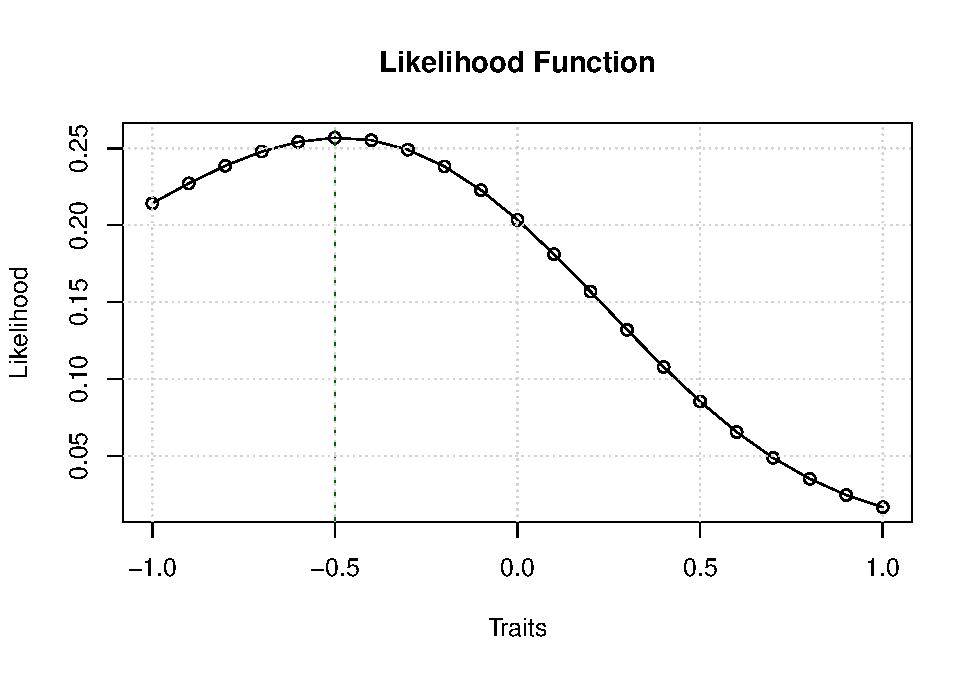
\includegraphics{Assignment_2_files/figure-latex/unnamed-chunk-7-1.pdf}
The plot shows that the maximum likelihood occurs at around
\(trait=-0.5\). The maximum likelihood is 0.26.

\end{document}
